\documentclass{article}

\usepackage{neurips_2026}
\makeatletter
\renewcommand{\@noticestring}{Submitted to the 2026 Conference on Physics and AI (PAI26). Do not distribute.}
\makeatother

\usepackage[utf8]{inputenc}
\usepackage[T1]{fontenc}
\usepackage{hyperref}
\usepackage{url}
\usepackage{booktabs}
\usepackage{amsmath}
\usepackage{amsfonts}
\usepackage{nicefrac}
\usepackage{microtype}
\usepackage{xcolor}
\usepackage{graphicx}
\usepackage{tikz}
\usetikzlibrary{shapes.geometric, arrows.meta, positioning, fit, backgrounds}

\title{LLM-Powered Automation of a Dark Matter Constraint Repository}

\begin{document}

\maketitle

\renewcommand{\thefootnote}{\fnsymbol{footnote}}
\footnotetext[1]{This paper was drafted with the assistance of large language models (Claude) under human supervision and editorial control.}
\renewcommand{\thefootnote}{\arabic{footnote}}
\setcounter{footnote}{0}

\begin{abstract}
Dark matter constraint repositories are critical community infrastructure, giving experimentalists and theorists a shared landscape of existing bounds. Yet the most widely-used repositories are maintained by individual volunteers, creating a sustainability risk as the pace of new results accelerates.
We present a large language model (LLM) pipeline that monitors arXiv, extracts limit curves from papers, integrates them as code, and opens pull requests (PRs) for human review.
On a 346-paper benchmark whose ground truth is the upstream-curated repository itself, the pipeline classifies the coupling type correctly for 90.5\% of papers and reaches a median coupling residual of 0.33~dex (a factor of two for 48\% of curves), with 76\% mean mass-range coverage.
Three design choices drive this: (i)~treating each extraction as a noisy sample and reconciling several reads by a consensus vote with source-quality tiering; (ii)~a convention-canonicalization layer whose per-file conversion factors were derived with a guided physics-derivation assistant (GPD), code-verified and citation-audited; and (iii)~a scoring methodology that separates genuine extraction error from non-comparability.
Strikingly, figure-vision extraction (0.34~dex) now matches text extraction (0.33~dex): reading log--log plots is no longer the bottleneck. The remaining difficulty is concentrated in rare coupling types with idiosyncratic conventions (macro-averaged residual 1.1~dex). The pipeline is deployed and has generated limit proposals; none have merged --- governance of AI-generated scientific data is itself an unsolved problem.
\end{abstract}

%----------------------------------------------------------------------
\section{Introduction}
%----------------------------------------------------------------------

The experimental search for ultralight dark matter is undergoing a ``renaissance''~\cite{snowmass_axion}, with new proposals targeting masses from $10^{-22}$~eV to several eV using techniques from quantum-limited cavities to dish antennas and nuclear magnetic resonance~\cite{irastorza_review, kim_review}.
The result is an ever-denser landscape of constraints across at least 15 distinct \emph{coupling types} (ways a dark matter candidate can interact with Standard Model particles, e.g.\ axion--photon or dark photon kinetic mixing)~\cite{dp_cookbook}, each with its own conventions for units, parameterisations, and confidence levels.

Dark matter constraint repositories compile these bounds into publication-quality \emph{exclusion plots} --- diagrams showing which regions of mass--coupling parameter space have been ruled out --- that appear in a large fraction of papers in the field~\cite{axionlimits, dp_cookbook, ohare_review}.
The AxionLimits repository~\cite{axionlimits} tracks over 600 limits and 160 projected sensitivities, yet is maintained by a single volunteer who must identify new results, extract data from figures or tables, convert between parameterisations (e.g.\ kinetic mixing $\chi$ vs.\ coupling $g$~\cite{dp_cookbook}), write plotting code, and regenerate figures.
With multiple relevant papers appearing weekly, this concentrates critical community infrastructure on a single point of failure.

We present a pipeline that partially automates this workflow: (1)~\textbf{Discovery} via daily arXiv monitoring with keyword filtering and LLM relevance classification; (2)~\textbf{Extraction} using a two-stage approach (text/tables first, vision fallback for plot-only papers) with multi-read consensus voting and a physics convention-canonicalization layer; (3)~\textbf{Integration} through automated code generation with Abstract Syntax Tree (AST)-based insertion, notebook updates, and plot regeneration; and (4)~\textbf{Review} via PRs with highlighted constraint plots.
The system also includes a weekly preprint version checker and a historical backfill workflow using INSPIRE-HEP~\cite{inspirehep}.\footnote{Code, evaluation benchmark, and prompts: \url{https://anonymous.4open.science/r/AutoAxionLimits-358C}}

\textbf{Related work.}
Chart understanding benchmarks (ChartQA~\cite{chartqa}, PlotQA~\cite{plotqa}) address visual QA but not numerical extraction from dense log--log exclusion plots; document parsers like GROBID~\cite{grobid} handle metadata, not figure digitisation. To our knowledge, no existing system automates the full loop from discovery through extraction, code integration, and human review for a live scientific repository.

\textbf{Contributions.}
(i)~An end-to-end pipeline that turns an arXiv paper into a reviewable code change for a real constraint repository. (ii)~An extraction stack that treats LLM reads as noisy samples and reconciles them by consensus with source-quality tiering, and pairs them with a physics convention-canonicalization layer whose conversions were established by a guided physics-derivation assistant rather than by prompting. (iii)~A 346-paper benchmark and scoring methodology that grounds truth in the upstream repository and separates extraction error from non-comparability. (iv)~The empirical finding that, with these in place, log--log plot reading is no longer the dominant error source --- the frontier shifts to deterministic, convention-bound rare coupling types.

%----------------------------------------------------------------------
\section{System Architecture}
%----------------------------------------------------------------------

Figure~\ref{fig:architecture} shows the end-to-end pipeline.

\begin{figure}[t]
\centering
\resizebox{0.66\textwidth}{!}{%
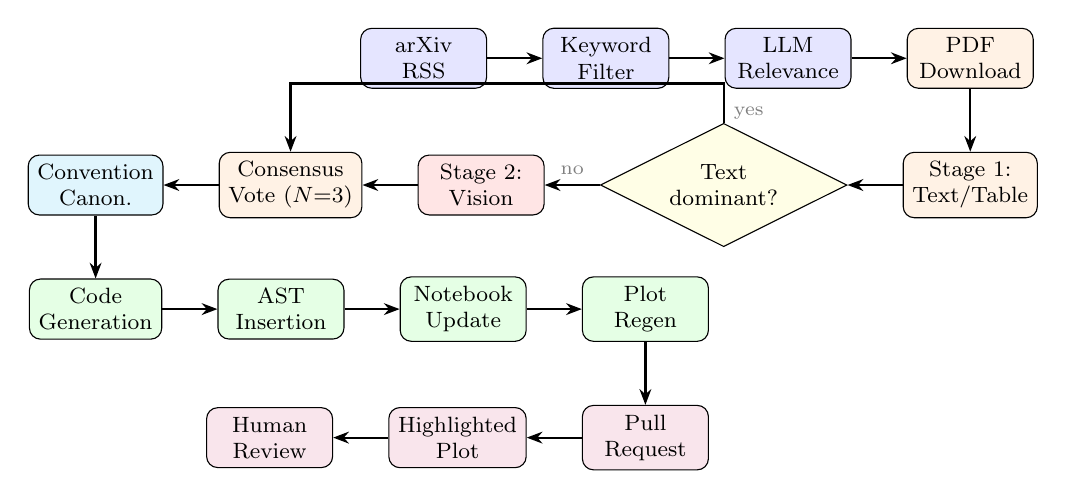
\begin{tikzpicture}[
    node distance=0.5cm and 0.7cm,
    block/.style={rectangle, draw, rounded corners, minimum height=0.7cm, minimum width=1.6cm, align=center, font=\footnotesize},
    decision/.style={diamond, draw, aspect=2, minimum width=1.0cm, align=center, font=\footnotesize},
    arrow/.style={-{Stealth[length=2mm]}, thick},
    label/.style={font=\scriptsize, text=gray},
]

% Row 1: Discovery
\node[block, fill=blue!10] (arxiv) {arXiv\\RSS};
\node[block, fill=blue!10, right=of arxiv] (kw) {Keyword\\Filter};
\node[block, fill=blue!10, right=of kw] (llm1) {LLM\\Relevance};
\node[block, fill=orange!10, right=of llm1] (pdf) {PDF\\Download};

% Row 2: Extraction (text/vision -> consensus -> convention)
\node[block, fill=orange!10, below=0.8cm of pdf] (text) {Stage 1:\\Text/Table};
\node[decision, fill=yellow!10, left=of text] (check) {Text\\dominant?};
\node[block, fill=red!10, left=of check] (vision) {Stage 2:\\Vision};
\node[block, fill=orange!10, left=of vision] (vote) {Consensus\\Vote ($N{=}3$)};
\node[block, fill=cyan!12, left=of vote] (conv) {Convention\\Canon.};

% Row 3: Integration
\node[block, fill=green!10, below=0.8cm of conv] (codegen) {Code\\Generation};
\node[block, fill=green!10, right=of codegen] (ast) {AST\\Insertion};
\node[block, fill=green!10, right=of ast] (notebook) {Notebook\\Update};
\node[block, fill=green!10, right=of notebook] (plot) {Plot\\Regen};

% Row 4: Review
\node[block, fill=purple!10, below=0.8cm of plot] (pr) {Pull\\Request};
\node[block, fill=purple!10, left=of pr] (highlight) {Highlighted\\Plot};
\node[block, fill=purple!10, left=of highlight] (human) {Human\\Review};

\draw[arrow] (arxiv) -- (kw);
\draw[arrow] (kw) -- (llm1);
\draw[arrow] (llm1) -- (pdf);
\draw[arrow] (pdf) -- (text);
\draw[arrow] (text) -- (check);
\draw[arrow] (check) -- node[above, label] {no} (vision);
\draw[arrow] (check.north) -- node[near start, right, label] {yes} ++(0,0.5) -| (vote.north);
\draw[arrow] (vision) -- (vote);
\draw[arrow] (vote) -- (conv);
\draw[arrow] (conv) -- (codegen);
\draw[arrow] (codegen) -- (ast);
\draw[arrow] (ast) -- (notebook);
\draw[arrow] (notebook) -- (plot);
\draw[arrow] (plot) -- (pr);
\draw[arrow] (pr) -- (highlight);
\draw[arrow] (highlight) -- (human);

\end{tikzpicture}
}
\caption{Pipeline architecture. Papers flow from arXiv through keyword and LLM filtering, two-stage extraction (text-first, vision fallback), multi-read consensus voting, physics convention canonicalization, code generation with AST-based insertion, plot regeneration, and finally a pull request with a highlighted constraint plot for human review.}
\label{fig:architecture}
\end{figure}

\subsection{Two-Stage Extraction with Consensus Voting}

The extraction pipeline prioritises text and table data (Stage~1) over vision-based figure reading (Stage~2), motivated by both cost and accuracy.

\textbf{Stage~1: Text and tables.}
The PDF is parsed with PyMuPDF~\cite{pymupdf} and the full text sent to an LLM~\cite{anthropic_claude} with a structured prompt requesting JSON output: coupling type, mass--coupling data points, the model's declared units/convention, and metadata. Prompt-injection defences strip control characters and wrap content in sentinel delimiters.

\textbf{Stage~2: Vision fallback.}
Vision is invoked only when Stage~1 is not \emph{clearly dominant} (a valid mass window, $\geq 5$ points, sufficient confidence, non-degenerate). Selected figure pages are rendered to images; the model reads axis labels, tick marks, and curve positions from log--log exclusion plots.

\textbf{Consensus across noisy reads.}
LLM extraction is non-deterministic, so each paper is read several times independently ($N{=}3$) and reconciled. The coupling type is chosen by majority vote; the reported curve is the \emph{medoid} --- the candidate with the smallest median pairwise distance to the others in log--log space. The medoid is a real sample, not an average, so consensus rejects one-off mis-reads without ever fabricating a non-physical curve by averaging incompatible ones.

\textbf{Quality-tier source selection.}
When candidates disagree, they are ranked by a lexicographic quality tuple rather than by raw point count: validity (values in physically allowed ranges), non-degeneracy (a traced curve must span $\geq 1$~dex, not a flat artefact), recoverability, \emph{source tier} (table $>$ text $>$ figure-vision), corroboration between reads, and confidence. A sparse text or table snippet ($\leq 3$ points, e.g.\ a headline bound quoted in prose) is demoted below a traceable multi-point figure curve, so a single quoted number cannot override an actual digitised constraint.

\subsection{Convention Canonicalization}
\label{sec:conv}

The same physics is reported in incompatible $y$-variables across papers and even across files within one coupling type, and the conversion often lives in the repository's plotting code, not in the paper. Examples we encountered: axion--nucleon couplings stored as the derivative coupling $g_{aNN}=C_N/2f_a$ [GeV$^{-1}$] but plotted dimensionless after an in-code $\times 2m_N$ (with a per-file $\times m_N$ exception for one detector); scalar/dilaton bounds stored as a genuine Damour--Donoghue $d_e\!\sim\!10^{-3}$ in some files but as a fifth-force strength $\alpha\!\sim\!10^{7}$ in others (related by $d_e=Q^{-1}\sqrt{\alpha}$, a $10$--$15$~dex \emph{apparent} offset that is not an error); dark-photon kinetic mixing reported as $\varepsilon^2$ vs.\ $\chi=\varepsilon$; and large sentinel values ($10^{20},10^{30},10^{99}$) that are \texttt{fill\_between} polygon-closing vertices, not data.

These are \emph{deterministic} mismatches: no amount of prompting fixes them, because the conversion depends on per-file repository storage that the paper never states. We encode them in a per-file convention registry that the comparator (and the production pipeline) applies to canonicalize both the extracted and reference curves before any residual is computed; values it cannot map are flagged \texttt{[CONVENTION REVIEW]} with capped confidence rather than emitted as a silent wrong number. Crucially, the conversion factors were not guessed: they were derived with a guided physics-derivation assistant (GPD), which produced a reference that is \emph{code-verified} against the repository's plotting source and notebooks and \emph{citation-audited} against the literature. Getting these right is a small but exacting physics task, and treating it as one --- rather than as a prompting problem --- is what made the registry trustworthy.

\subsection{Code Generation, Integration, and Review}

The LLM generates a \texttt{@staticmethod} for the relevant plotting class (a post-generation guard enforces the decorator); insertion uses Python's AST module to locate the last method in the target class --- never regex --- preventing corruption. Notebook cells are inserted via \texttt{nbformat} and plots regenerated headlessly via \texttt{nbconvert}. Every update becomes a pull request, with low-confidence or unresolved-convention extractions flagged in the title. Crucially, we render a ``highlighted'' constraint plot in which all existing limits are greyed out and only the new proposed limit is shown in red (Figure~\ref{fig:highlighted}), enabling rapid visual verification by domain experts without reading code.

\begin{figure}[t]
\centering
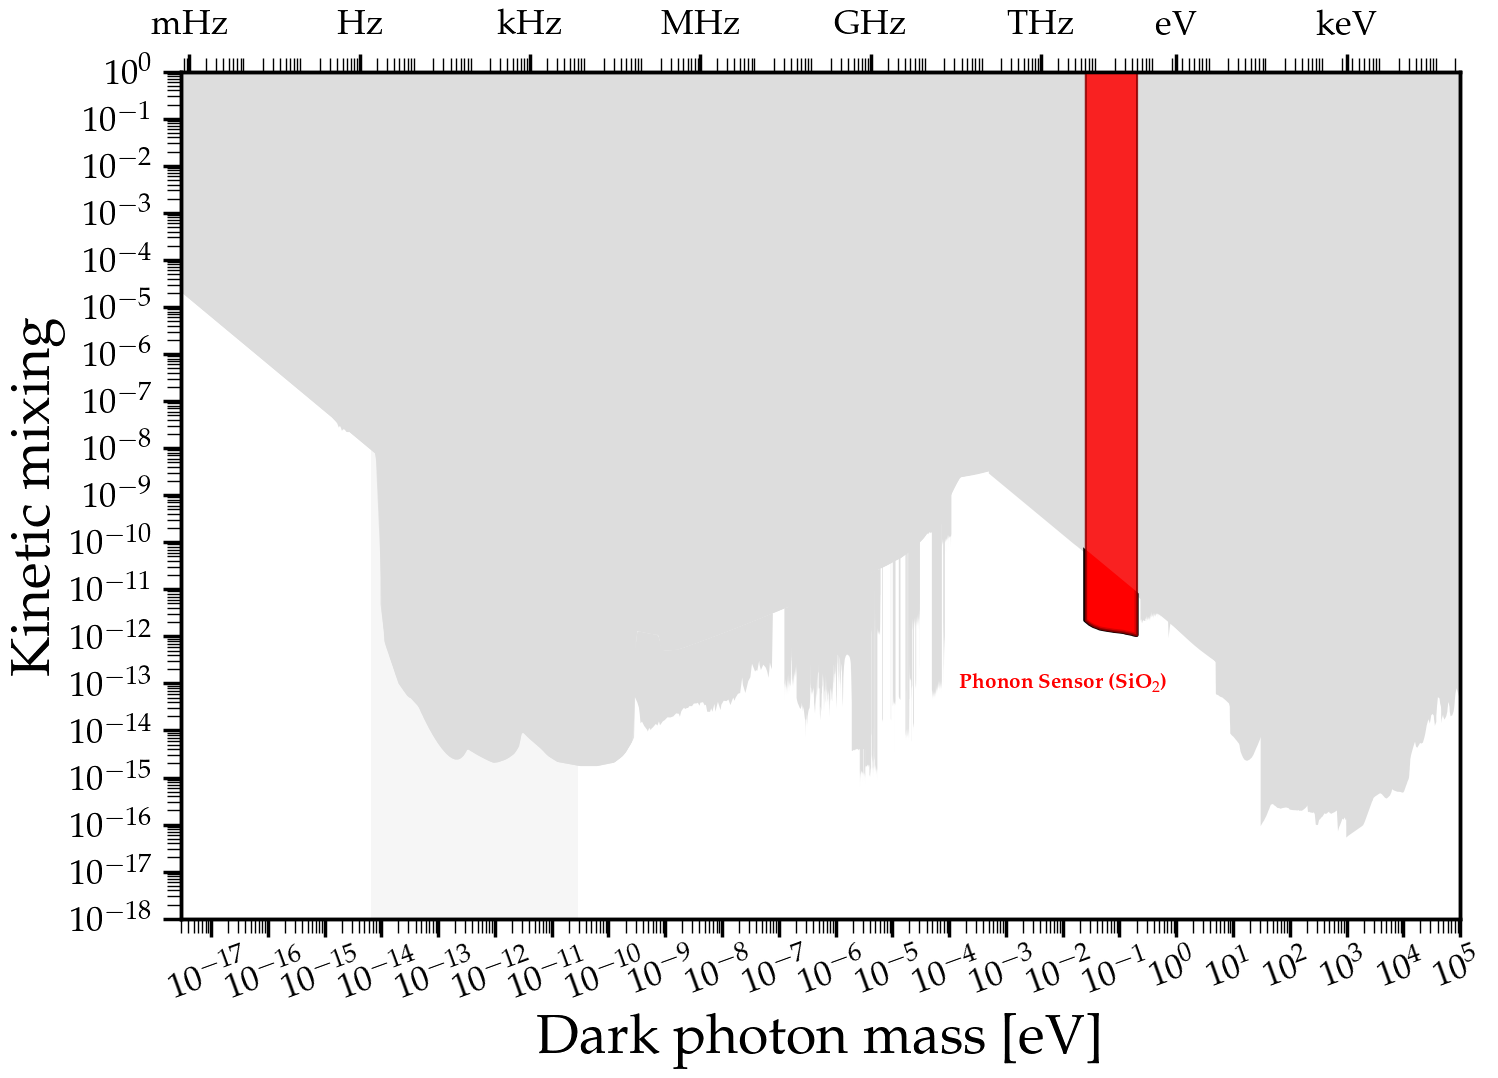
\includegraphics[width=0.5\textwidth]{figures/DarkPhoton_highlighted.png}
\caption{Highlighted dark photon constraint projection plot from a production pull request for a phonon-sensor proposal~\cite{phonon_sensor}. Existing limits in grey; new proposal in red. This format lets reviewers verify the proposal visually.}
\label{fig:highlighted}
\end{figure}

\subsection{Workflows and Cost}

The \textbf{daily arXiv digest} queries, filters, classifies relevance, and processes matching papers. The \textbf{weekly preprint checker} scans existing data files for arXiv IDs and re-extracts on version updates to catch changed results; one PR detected that a JWST dark photon search~\cite{jwst_dp} had changed a limit to a projection upon publication. The \textbf{historical backfill} searches INSPIRE-HEP~\cite{inspirehep} for older papers by citation count, splitting large jobs across daily runs.

The pipeline runs on a frontier model (Claude Opus~\cite{anthropic_claude}) to maximise extraction quality. With $N{=}3$ consensus and conditional vision, a paper triggers roughly five to nine model calls; text-only papers (the majority) avoid expensive image tokens. We do not present this as a cheap pipeline --- per-paper cost is on the order of tens of cents to a few dollars, dominated by vision papers --- but it remains far below the expert time it substitutes for, and text-first gating bounds the spend.

%----------------------------------------------------------------------
\section{Evaluation}
\label{sec:eval}
%----------------------------------------------------------------------

\textbf{Benchmark and ground truth.}
We evaluate on 346 papers spanning 14 coupling types, selected as all curated data files~\cite{axionlimits} with a known arXiv ID. The ground truth for each is the upstream repository's own digitised curve --- never data digitised by our own model --- which avoids circularity but carries a consequence: the reference was itself digitised and rescaled from the same papers, so a \emph{perfect} extraction still shows a nonzero residual equal to the upstream digitisation/convention gap. Our reported residuals are therefore an \emph{upper bound} on true extraction error.

\textbf{Metric.}
We compare in $\log_{10}$--$\log_{10}$ space: a log--log interpolation is built from the extracted points and evaluated at ground-truth masses, giving a per-point residual $|\log_{10} g_\text{ext} - \log_{10} g_\text{truth}|$ (0.3~dex $\approx$ factor of 2). We report median residual and \emph{interpolation coverage} (fraction of GT masses the extracted curve spans) separately, because a curve can be accurate where it overlaps yet cover the wrong mass window. A reverse pass (GT interpolated onto the extracted masses) flags curves that run past the true mass range.

\textbf{Honest disposition taxonomy.}
A curve is scored only against a same-coupling GT curve; we partition the rest so non-comparability never pollutes the residual statistics: \emph{no comparable GT} (30 papers; predicted coupling absent, usually a misclassification), \emph{convention mismatch} (10; same coupling, incompatible parameterisation), \emph{point reference} (14; GT is a single operating-point limit, not a curve), \emph{no extracted points} (16), and \emph{no prediction} (3). Of 346 papers, 271 are comparable; the residual statistics below are over those.

\textbf{Classification labels.}
Coupling type is scored against the repository's directory structure. The property labels (\emph{is new limit}, \emph{is projection}, \emph{data source}) are scored against an \emph{independent} LLM labeler (a different model and prompt from the extractor it grades), making this a cross-model check rather than self-agreement; a 15-paper human audit found labeler--human agreement of 15/15, 15/15, and 14/15 on the three fields.

\begin{table}[t]
\caption{Benchmark performance on 346 papers. Residual statistics are over the 271 comparable papers (243 with mass-range overlap); $0.3$~dex $\approx$ a factor of two.}
\label{tab:results}
\centering
\small
\begin{tabular}{@{}lc@{\hskip 2em}lcc@{}}
\toprule
\textbf{Aggregate metric} & \textbf{Value} & \textbf{By source / pooling} & \textbf{Med.\ resid.} & \textbf{$\leq$0.3 dex} \\
\midrule
Coupling-type accuracy & 90.5\% & Text ($N{=}148$)        & 0.326 dex & 49.7\% \\
Median residual         & 0.331 dex & Figure-vision ($N{=}119$) & 0.338 dex & 46.8\% \\
Within factor 2         & 48.4\% & Micro-avg (per paper)   & 0.331 dex & 48.4\% \\
Within factor 3         & 61.7\% & Macro-avg (per type)    & 1.115 dex & --- \\
Mean interp.\ coverage  & 76.2\% & \quad AxionPhoton ($N{=}127$) & 0.207 dex & --- \\
Zero-overlap papers     & 10.3\% & \quad AxionEDM ($N{=}3$) & 4.649 dex & --- \\
\bottomrule
\end{tabular}
\end{table}

\textbf{Results.}
Table~\ref{tab:results} summarises the benchmark. Coupling-type classification is reliable (90.5\%); 90\% of comparable papers achieve mass-range overlap, with a median residual of 0.33~dex and 48\% of curves within a factor of two, at 76\% mean coverage. The reverse pass agrees (median 0.34~dex), indicating the curves cover the right mass extent, not just the right values where they overlap.

The most consequential result is the \emph{source breakdown}: figure-vision extraction (0.338~dex, 46.8\% within factor two) is now on par with text extraction (0.326~dex, 49.7\%). Reading dense log--log plots --- historically the hard part of this task --- is no longer the limiting factor; consensus voting and quality-tier selection over multiple reads close most of the figure-vision gap.

\textbf{Where the difficulty now lives.}
The frontier has shifted to \emph{rare coupling types}. The per-paper micro-average (0.33~dex) is dominated by the most common type (AxionPhoton, 0.21~dex, $N{=}127$); the per-type macro-average is 1.1~dex. Common types are strong (DarkPhoton 0.41, AxionElectron 0.38), but small-sample, convention-heavy types lag: AxionNeutron 0.77, VectorBL 0.91, AxionMass 0.94, and AxionEDM 4.6~dex. AxionEDM is the clearest case: the operator coupling $g_{a\gamma\gamma\gamma}$ is flat in mass while the experimentally reported \emph{response} $\propto 1/m_a$ folds in the field amplitude --- a convention our registry flags but does not yet auto-convert. These types also concentrate the coupling-type misclassifications, so they compound: a wrong type is scored against the wrong reference.

\textbf{Yardsticks.}
Two floors bound interpretation. The run-to-run LLM \emph{noise floor} (90th-percentile per-paper residual std over repeated extractions) is 0.32~dex --- consensus voting is what keeps most papers inside it. The upstream \emph{digitisation floor} (truly independent re-digitisation vs.\ repo, table/text sources) is only $\sim$0.03~dex, so the residuals we report are real extractor error, not a yardstick artefact, and the median sits essentially at the noise floor.

%----------------------------------------------------------------------
\section{Lessons Learned}
%----------------------------------------------------------------------

\textbf{Treat extraction as noisy and vote.}
A single LLM read of a log--log plot is unreliable and irreproducible. Reading each paper $N{=}3$ times and reconciling by a medoid consensus with source-quality tiering was the single change that moved figure-vision from the dominant failure mode to parity with text. The medoid matters: averaging incompatible curves would manufacture a non-physical bound, whereas the medoid returns a real, central sample.

\textbf{The worst errors are deterministic physics, not perception --- solve them with verified derivation.}
The largest residuals were never about pixels. They were unit/convention mismatches --- the axion--nucleon $2m_N$ factor, the scalar $d_e$ vs.\ $\sqrt{\alpha}$ $10$--$15$~dex gap, dark-photon $\varepsilon$ vs.\ $\varepsilon^2$, sentinel values mistaken for data --- that are fixed, not stochastic, and depend on per-file repository conventions absent from the paper. The high-leverage fix was not a better prompt but a separate, auditable physics layer: we used a guided physics-derivation assistant (GPD) to produce a \emph{code-verified, citation-audited} per-file convention registry, turning ``unsafe guessing'' about conversion factors into vetted closed-form maps, with a \texttt{[CONVENTION REVIEW]} flag for anything outside the verified set. Canonicalizing both sides before scoring also let us report \emph{convention mismatch} as its own disposition (10 papers) instead of as inflated error. The general lesson for automated scientific extraction: it couples a \emph{stochastic} perception problem (reading plots, best handled by sampling and voting) with a \emph{deterministic} domain-knowledge problem (conventions, best handled by verified derivation), and the two demand different tools.

\textbf{Score honestly.}
Grounding truth in the upstream repository (never in our own model's digitisation) avoids circularity and makes the residual a defensible upper bound. Separating non-comparability (wrong-coupling, point-reference, convention-mismatch) from genuine error keeps the headline numbers meaningful, and scoring property labels against an independent LLM labeler rather than placeholders restores those metrics as a fair cross-model test.

\textbf{Engineering that paid off.}
Text-first extraction with conditional vision keeps the majority of papers off the expensive vision path; AST-based insertion produces syntactically valid methods; and highlighted plots make review accessible to non-coders.

\textbf{What is still hard.}
Rare coupling types remain the open problem: small samples, idiosyncratic conventions (the AxionEDM operator-vs-response case, scalar fifth-force files), and the misclassifications that send them to the wrong reference. At 90\% coupling accuracy roughly one proposal in ten still targets the wrong plot, so human-in-the-loop review is essential, not optional. A residual $\sim$10\% of papers also miss the mass window entirely (too few points or the wrong panel).

\textbf{Governance.}
The pipeline is deployed and has generated limit proposals; none have merged, because no review process for AI-generated scientific data exists. We recommend a community editorial board analogous to PDG reviewers~\cite{pdg}, where collaborations validate their own limits. More fundamentally, publishing machine-readable limit data alongside papers would bypass the extraction bottleneck altogether --- the highest-leverage change the field could make.

%----------------------------------------------------------------------
% References
%----------------------------------------------------------------------

\bibliographystyle{unsrt}

\begin{thebibliography}{18}

\bibitem{snowmass_axion}
C.~B.~Adams et~al.,
``Axion dark matter,''
in \textit{Snowmass 2021}, arXiv:2203.14923, 2022.

\bibitem{irastorza_review}
I.~G. Irastorza and J.~Redondo,
``New experimental approaches in the search for axion-like particles,''
\textit{Prog. Part. Nucl. Phys.} \textbf{102}, 89, 2018.

\bibitem{kim_review}
J.~E. Kim and G.~Carosi,
``Axions and the strong CP problem,''
\textit{Rev. Mod. Phys.} \textbf{82}, 557, 2010.

\bibitem{dp_cookbook}
A.~Caputo, A.~J.~Millar, C.~A.~J.~O'Hare, and E.~Vitagliano,
``Dark photon limits: a handbook,''
\textit{Phys. Rev. D} \textbf{104} (9), 095029, 2021,
arXiv:2105.04565~[hep-ph].

\bibitem{axionlimits}
C.~A.~J. O'Hare,
``AxionLimits,''
\url{https://github.com/cajohare/AxionLimits}, 2020.

\bibitem{ohare_review}
C.~A.~J. O'Hare,
``Cosmology of axion dark matter,''
\textit{PoS} \textbf{COSMICWISPers}, 040, 2024.

\bibitem{inspirehep}
INSPIRE Collaboration,
``INSPIRE-HEP: High-Energy Physics Literature Database,''
\url{https://inspirehep.net}, 2024.

\bibitem{anthropic_claude}
Anthropic,
``The Claude model family,''
\url{https://www.anthropic.com}, 2024.

\bibitem{chartqa}
A.~Masry, D.~X. Long, J.~Q. Tan, S.~Joty, and E.~Hoque,
``ChartQA: A Benchmark for Question Answering about Charts with Visual and Logical Reasoning,''
\textit{Findings of ACL}, 2022.

\bibitem{plotqa}
N.~Methani, P.~Ganguly, M.~M.~Khapra, and P.~Kumar,
``PlotQA: Reasoning over Scientific Plots,''
\textit{WACV}, 2020.

\bibitem{grobid}
P.~Lopez,
``GROBID: GeneRation Of BIbliographic Data,''
\url{https://github.com/kermitt2/grobid}, 2008--2024.

\bibitem{pymupdf}
Artifex Software,
``PyMuPDF,''
\url{https://github.com/pymupdf/PyMuPDF}, 2015--2025.

\bibitem{jwst_dp}
H.~An, S.~Ge, J.~Liu, and Z.~Lu,
``Direct Detection of Dark Photon Dark Matter with the James Webb Space Telescope,''
arXiv:2402.17140, 2024.

\bibitem{phonon_sensor}
I.~M.~Bloch, S.~Knapen, X.~Li, A.~Madden, and G.~Marocco,
``Dark Matter Detection Using Phonon Sensing in Amorphous Materials,''
arXiv:2603.22390, 2026.

\bibitem{pdg}
S.~Navas et~al. (Particle Data Group),
``Review of particle physics,''
\textit{Phys.\ Rev.\ D} \textbf{110} (3), 030001, 2024.

\end{thebibliography}

\end{document}
